\section{Results}

\begin{figure}[h]
    \centering
    \includegraphics[width=0.45\linewidth]{analysis/artefact/variation_approach/reduction_query_execution_time}
    \caption{
        This figure compares the type index with the LDP approach against other approaches.
        The shape index approach performs better generarly than the other approaches except with S4.
        The shape index can also answer queries from the S7V3, which the plot cannot capture.
    }
    \label{fig:compApproach}
\end{figure}


Figure~\ref{fig:compApproach} shows that the shape index can, with multiple queries, perform better or comparably to the state-of-the-art (type index with LDP approach), with queries requiring as little as 13\% (S1) of the execution time.
The queries that perform best are those where the number of HTTP requests decreased the most.
The Appendix displays plots of the number of HTTP requests by query template and presents the statistical significance for each query instance.
Query templates D6 and D7 show no reduction because they require nearly every document in the dataset to be processed by the engine, making our approach ineffective in these cases.
We notice that query template S4 with the shape index performed worse in every instance, with an increase in query execution time of up to 2.80 times.
The poor performance is due to the fact that other approaches rely solely on the reachability \texttt{Cmatch} to achieve completeness, without leveraging the structural properties of the dataset. 
In contrast, the shape index approach always enforces the use of these properties, resulting in additional HTTP requests and increased processing time.
This is further illustrated in Table~\ref{tab:ratioUsefulResources}, which shows that for these queries, the state-of-the-art achieves a ratio of useful resources dereferenced of 100\% or 50\%, compared to only 6\% with the shape index approach.
However, those queries were already fast, with the state-of-the-art approach being executed in approximately 0.30\% of the timeout.
Nonetheless, these results still highlight a category of queries and networks for which our approach is not well-suited.

The empirical evaluation of the query-containment algorithm shows that its execution with the more detailed shapes of our experiment is negligible, with a maximum execution of 4.655 ms (0.0039\% of the timeout), as presented in table~\ref{tab:queryShapeContainmentEval}.
This result is expected because the algorithm's time complexity is ("TO INSERT"), and the experiments' shapes and queries are small, not deeply nested instances.
This shows that most of the overhead for this approach is not this algorithm but is probably the state retention for the pruning reachability criteria in the form of filters in the link queue.

\begin{figure}[htbp]
    \centering
    % First figure
    \begin{minipage}[t]{0.45\textwidth}
        \centering
        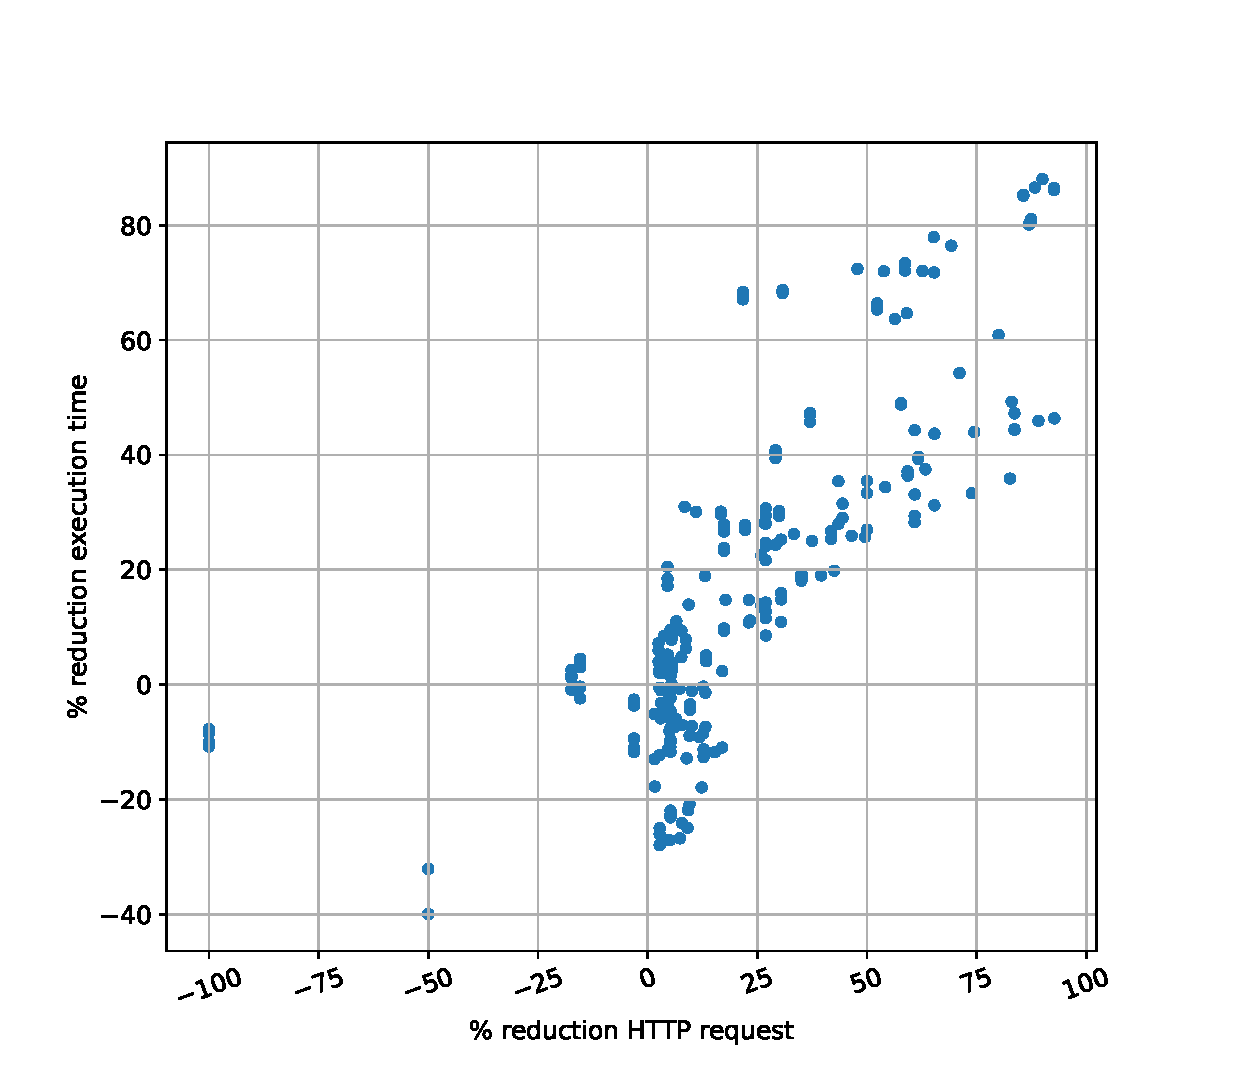
\includegraphics[width=\linewidth]{analysis/artefact/http_req_exec_time_relation/http_req_exec_time_cor_better}
        \label{fig:http_req_exec_time_cor_better}
    \end{minipage}
    \hspace{0.05\textwidth}
    % Second figure
    \begin{minipage}[t]{0.45\textwidth}
        \centering
        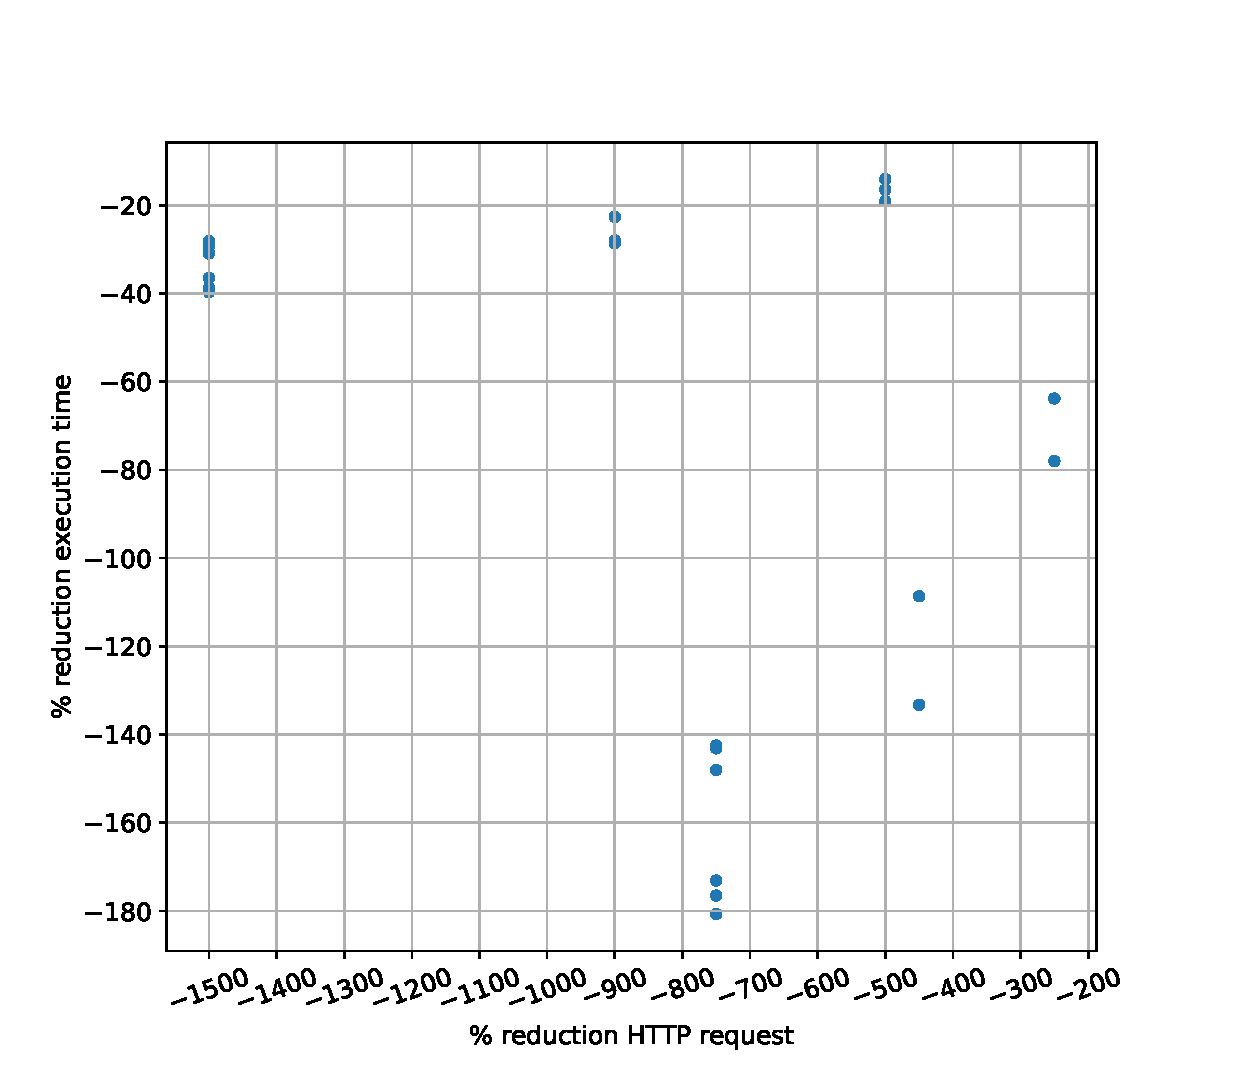
\includegraphics[width=\linewidth]{analysis/artefact/http_req_exec_time_relation/http_req_exec_time_cor_worse}
        \label{fig:http_req_exec_time_cor_worse}
    \end{minipage}

    % General caption
    \caption{
        The data show two regimes in the relation between the number of HTTP requests and the execution time, 
        we see a more linear correlation on the left figure than on the right figure.
        %The overall distribution is linear, with a PCC of 0.55 and a p-value of 6.18E-35.
        }
    \label{fig:http_req_exec_time_cor}
\end{figure}

To determine the relationship between the reduction of HTTP requests and the query execution time, we evaluated their ratio using 
the data of our experiments with the state-of-the-art results, the type index, and the LDP specification as the baseline.
This analysis is reported through Figure~\ref{fig:http_req_exec_time_cor}.
The relationship between HTTP request and query execution time can be divided into two regimes.
In the first regime (left figure), where the shape index approach reduces the number of HTTP requests, we notice a positive linear correlation with a
Pearson correlation coefficient (PCC) of 0.83 and a high statistical significance given a p-value of 2.94E-93.
We also notice that below a ratio of approximately 0.83 of HTTP requests, the shape index approach did not guarantee a reduction in query execution time.
In the second regime (right figure), the shape index increases the number of HTTP requests.
We notice a weaker positive linear correlation with a PCC of 0.43 and a high but far lower statistical significance given a p-value of 1.16E-04.
The overall correlation between reducing HTTP requests and query execution time is positively linear, with a PCC of 0.55 and a high statistical significance with a p-value of 6.18E-35.
It is difficult to explain why the data operate in two regimes. 
A possible explanation can be the lack of samples when the shape index approach performs poorly.
However, we can also notice that the relationship between the two variables in the first regime is closer to one-on-one than in the second regime, where the ratio of HTTP requests has less of an impact.
This observation can lead us to question how complex the queries are in that regime; we can notice that the queries where the shape index increases vastly in the number 
of HTTP requests are the queries from the S4 template. 
However, this query was already answered quickly and consisted of only four triple patterns and a union statement (with the alternative property path), so the query is simple. 
Thus, it is possible that the number of HTTP requests has less of an impact because it is easier for the engine to perform the join operation upon reception of the data than when processing more complex queries.
With this current experiment and data, it is impossible to give a conclusive answer.

\begin{figure}[htbp]
    \centering
    % First figure
    \begin{minipage}{0.32\textwidth}
        \centering
        \includegraphics[width=\linewidth]{analysis/artefact/variation_percentage_shape_index/reduction_query_execution_time}
        \caption*{a) Percentage of shape index in the network}
        \label{fig:varPercentShapeIndex}
    \end{minipage}
    \hfill
    % Second figure
    \begin{minipage}{0.32\textwidth}
        \centering
        \includegraphics[width=\linewidth]{analysis/artefact/variation_percentage_entry_shape_index/reduction_query_execution_time}
        \caption*{b) Percentage of entries having open shapes}
        \label{fig:varPercentEntries}
    \end{minipage}
    \hfill
    % Third figure
    \begin{minipage}{0.32\textwidth}
        \centering
        \includegraphics[width=\linewidth]{analysis/artefact/variation_detail_shape/reduction_query_execution_time}
        \caption*{c) Level of detail of the shapes}
        \label{fig:varShapeDetail}
    \end{minipage}

    % General caption
    \caption{Setups with less shape index information tend to perform worse where the shape index perform
    better against the other approaches in similar relative proportions.
    %We also observe that having a higher percentage of open shapes have generally a less negative impact than 
    %on performance compared to having a lower percentage of datasets without shape indexes.
    }
    \label{fig:adaptShapeIndex}
\end{figure}

The last part of the results analysis is the shape index's approach adaptivity.
For this analysis, we analyze what happens when we reduce the shape index information in the network and compare the results,
with a network with shape indexes and complete information.
In Figure~\ref{fig:adaptShapeIndex} a) and b), we can observe the expected results on queries 
where the shape index performed better, reducing the amount of information in the network reduced performance,
on queries where it had little impact, it still has little impact, and on the queries of S4, it improved performance.
We can also observe that having an incomplete shape index in the network generally impacts performance less than
missing shape indexes, which is also an intuitive result.
With plot c), we see that the level of detail of the shape of the shape index for most queries does not have much negative impact on performance and can even be improved.
Most queries do not necessitate complete information about the data model to discriminate sources, and for our experiment, each shape
had its own resource; thus, more detailed shapes can necessitate more HTTP requests to obtain the full information.
Query template S1 behaves differently from the other queries because more information about the data model was needed to perform a similar source selection than our baseline
which led to an increase in execution time of up to 9 times.
Looking back at b), the approach with 80\% of the entries completed performed much worse, which seems counterintuitive.
However, with the understanding that S1 is highly sensitive to the level of detail of the shape (notice that the lost of performance is also around nine times) and considering that 
the missing entries were assigned randomly;
we have five instances for each query;
It was a chance that led to incomplete entries being the most impactful for source selection for one query.
Additionally, with this experiment, even if a shape index is dereferenced with all its associated shapes, there is no guarantee that
the entry necessary for better source selection is present, which can, in some circumstances, lead to a higher loss of performance than
with the experiment of a).
